% Editable shared illustration: reading PDF, print, EPUB, online reader.
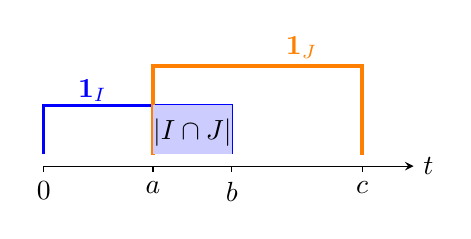
\begin{tikzpicture}[scale=0.77,>=stealth]
\draw[->] (0,0)--(6.1,0) node[right] {$t$};
\draw[very thick,blue] (0,.2)--(0,1)--(3.1,1)--(3.1,.2);
\draw[very thick,orange] (1.8,.18)--(1.8,1.65)--(5.25,1.65)--(5.25,.18);
\fill[blue!20] (1.8,.2) rectangle (3.1,1);
\node at (2.45,.56) {$|I\cap J|$};
\node[blue] at (.8,1.25) {$\mathbf1_I$};
\node[orange] at (4.25,1.95) {$\mathbf1_J$};
\foreach \x/\lab in {0/0,1.8/a,3.1/b,5.25/c}{\draw (\x,0)--(\x,-.1) node[below] {$\lab$};}
\end{tikzpicture}
